\subsection{Caso de Prueba 4 — Trío no colineal con intruso rasante}

El cuarto experimento explora la dinámica de una binaria estelar que sufre la irrupción de un tercer cuerpo masivo que ingresa con trayectoria casi tangencial.\ La configuración, basada en el cuaderno \emph{``Trío no colineal con planeta errante''}, busca emular encuentros cercanos en cúmulos abiertos donde un objeto errante puede transferir energía y modificar de forma radical la estabilidad de la pareja inicial.

El sistema se integra en unidades astronómicas (UA, años, masas solares) y utiliza el integrador \texttt{IAS15} de REBOUND para capturar fenómenos caóticos.\ La documentación que sigue detalla los parámetros de entrada, las celdas principales del notebook y los artefactos generados para su análisis posterior.

\paragraph{A. Propósito}
Medir cómo la heurística híbrida (algoritmo genético más refinamiento continuo) puede reducir el exponente de Lyapunov y contener la dispersión orbital cuando un intruso de masa intermedia atraviesa el plano orbital de la binaria. El objetivo es encontrar una combinación de masas que mantenga al intruso cautivo o, al menos, desacelere la divergencia de trayectorias respecto al estado inicial.

\paragraph{B. Parámetros críticos del escenario}
El diccionario \texttt{case} (Listing~\ref{lst:c04_case}) define horizontes de integración, condiciones iniciales y límites de búsqueda. Los valores fueron elegidos para propiciar inestabilidad sin caer en integraciones prohibidamente costosas.

\begin{listing}[H]
\caption{Declaración del diccionario \texttt{case} en el notebook Caso04}
\label{lst:c04_case}
\begin{adjustbox}{max width=\textwidth}
\begin{minipage}{\textwidth}
\begin{minted}[fontsize=\small, breaklines, breakanywhere]{python}
# Tres cuerpos caótico (unidades físicas)
case = {
    # Integración (UA, años, masas solares)
    "t_end_short": 0.6,             # ~1.4 periodos de la binaria
    "t_end_long": 3.5,              # ventana larga para ver la dispersión
    "dt": 2.0e-4,                   # aprox 0.073 días; suficiente para IAS15
    "integrator": "ias15",

    # Condiciones iniciales: binaria compacta + intruso
    "r0": (
        (-0.2916667, 0.0, 0.0),     # estrella primaria (~1.05 Msun)
        (0.4083333, 0.0, 0.0),      # estrella secundaria (~0.75 Msun)
        (0.0, 1.8, 0.0),            # intruso (planeta/brown dwarf)
    ),
    "v0": (
        (0.0, -4.19812977, 0.0),    # velocidad orbital de la primaria
        (0.0, 5.87738168, 0.0),     # velocidad orbital de la secundaria
        (-3.2, 0.0, 0.0),           # intruso con trayectoria rasante
    ),

    # Rangos de masa físicos pero amplios (fomenta caos)
    "mass_bounds": (
        (1.00, 1.50),               # estrella mayor tipo G
        (0.5, 1.0),                 # estrella secundaria tipo K
        (5e-5, 5e-1),               # planeta masivo / enano marrón
    ),
    "G": 39.47841760435743,         # 4pi^2 en unidades astronómicas
    "periodicity_weight": 0.02,     # penalización suave delta(r) + delta(v)

    # GA / búsqueda continua
    "pop_size": 180,
    "n_gen_step": 5,
    "crossover": 0.85,
    "mutation": 0.20,
    "elitism": 2,
    "seed": 98765,

    # Control de ejecución (rápido pero con margen)
    "max_epochs": 50,
    "top_k_long": 12,
    "stagnation_window": 5,
    "stagnation_tol": 1.25e-4,
    "local_radius": 0.04,
    "radius_decay": 0.85,
    "time_budget_s": 1800.0,
    "eval_budget": 16000,

    # Artefactos / salida
    "artifacts_dir": "artifacts/caso04_caotico",
    "save_plots": True,
    "headless": False,
}
\end{minted}
\end{minipage}
\end{adjustbox}
\end{listing}

\begin{table}[H]
\centering
\caption{Resumen de parámetros críticos del Caso 04}
\label{tab:c04_params} %chktex 24
\begin{tabularx}{\textwidth}{@{}l>{\raggedright\arraybackslash}X@{}}
\toprule
\textbf{Componente} & \textbf{Descripción} \\
\midrule
Horizontes e integrador & $t_{\text{short}} = 0.6$ años, $t_{\text{long}} = 3.5$ años, paso $\Delta t = 2\times10^{-4}$ años, integrador \texttt{IAS15}. \\
Condiciones iniciales & Binaria en el eje X con separaciones de $0.700$ UA;\ intruso arriba del plano a $1.8$ UA con impulso tangencial $-3.2$ UA/año. \\
Rangos de masa & Primaria $[1.0, 1.5]$ M$_\odot$, secundaria $[0.5, 1.0]$ M$_\odot$, intruso $[5\times 10^{-5}, 5\times 10^{-1}]$ M$_\odot$. \\
Penalización & \texttt{periodicity\_weight} $= 0.02$ mantiene énfasis en trayectorias contrastando dispersión vs.\ periodicidad. \\
Heurística evolutiva & Población 180, cruce $0.85$, mutación $0.20$, elitismo 2, radio local inicial $0.04$ con decaimiento $0.85$. \\
Presupuesto & $50$ épocas, máximo $16000$ evaluaciones, ventana de estancamiento 5 épocas y presupuesto temporal de $1800$ s. \\
Artefactos & Resultados persistidos en \texttt{artifacts/caso04\_caotico}, visualizadores en modo interactivo (\texttt{headless} = False). \\
\bottomrule
\end{tabularx}
\end{table}

\paragraph{C. Anatomía del notebook (celdas de código)}
Las secciones siguientes describen cada celda de código del cuaderno. Las celdas de markdown sirven como narrativa de soporte; aquí se documenta el flujo reproducible, los parámetros utilizados y las salidas relevantes.

\subsubsection*{Celda 3 — Preparación de rutas}
\paragraph{Descripción} Localiza la raíz \texttt{two\_body}, la inyecta en \texttt{sys.path} y aborta si no logra encontrarla. Es el mismo utilitario usado en los casos anteriores, necesario para importar paquetes locales cuando el notebook se ejecuta fuera del entorno del repositorio.
\paragraph{Código}
\begin{listing}[H]
\caption{Celda 3: detección de la raíz del proyecto}
\label{lst:c04_cell03}
\begin{adjustbox}{max width=\textwidth}
\begin{minipage}{\textwidth}
\begin{minted}[fontsize=\small, breaklines, breakanywhere]{python}
import sys
from pathlib import Path
PROJECT_ROOT = Path.cwd().resolve()
while PROJECT_ROOT.name != 'two_body' and PROJECT_ROOT.parent != PROJECT_ROOT:
    PROJECT_ROOT = PROJECT_ROOT.parent
if PROJECT_ROOT.name != 'two_body':
    raise RuntimeError('No se encontró la carpeta two_body')
PARENT = PROJECT_ROOT.parent
if str(PARENT) not in sys.path:
    sys.path.insert(0, str(PARENT))
print('PYTHONPATH += ', PARENT)
\end{minted}
\end{minipage}
\end{adjustbox}
\end{listing}
\paragraph{Salida} Mensaje que confirma la ruta añadida.

\subsubsection*{Celda 5 — Dependencias principales}
\paragraph{Descripción} Carga clases de configuración, controlador híbrido, visualizadores 2D/3D y el adaptador de REBOUND.\ También importa \texttt{NumPy} y \texttt{Path} para persistir artefactos.
\paragraph{Código}
\begin{listing}[H]
\caption{Celda 5: importación del pipeline principal}
\label{lst:c04_cell05}
\begin{adjustbox}{max width=\textwidth}
\begin{minipage}{\textwidth}
\begin{minted}[fontsize=\small, breaklines, breakanywhere]{python}
from two_body import Config, set_global_seeds
from two_body.core.telemetry import setup_logger
from two_body.logic.controller import ContinuousOptimizationController
from two_body.presentation.visualization import Visualizer as PlanarVisualizer
from two_body.presentation.triDTry import Visualizer as Visualizer3D
from two_body.simulation.rebound_adapter import ReboundSim
import numpy as np
from pathlib import Path
\end{minted}
\end{minipage}
\end{adjustbox}
\end{listing}
\paragraph{Salida} Sin salida; cualquier excepción revelaría dependencias ausentes.

\subsubsection*{Celda 7 — Instrumentación de rendimiento}
\paragraph{Descripción} Activa la captura de timings (\texttt{PERF\_TIMINGS\_ENABLED=1}) y expone utilidades para leer los CSV generados por la suite de mediciones.
\paragraph{Código}
\begin{listing}[H]
\caption{Celda 7: configuración de \texttt{perf\_timings}}
\label{lst:c04_cell07}
\begin{adjustbox}{max width=\textwidth}
\begin{minipage}{\textwidth}
\begin{minted}[fontsize=\small, breaklines, breakanywhere]{python}
import os
os.environ['PERF_TIMINGS_ENABLED'] = '1'
os.environ.setdefault('PERF_TIMINGS_JSONL', '0')
from two_body.perf_timings.timers import time_block
from two_body.perf_timings import latest_timing_csv, read_timings_csv, parse_sections_arg, filter_rows
\end{minted}
\end{minipage}
\end{adjustbox}
\end{listing}
\paragraph{Salida} No produce salida directa; modifica el entorno del proceso.

\subsubsection*{Celda 9 — Logging adaptado a notebook}
\paragraph{Descripción} Define un \texttt{NotebookHandler} que acumula los mensajes y los imprime en la misma celda, facilitando el seguimiento del optimizador sin recurrir a archivos externos. Ajusta el logger global al nivel \texttt{INFO}.
\paragraph{Código}
\begin{listing}[H]
\caption{Celda 9: configuración de logs interactivos}
\label{lst:c04_cell09}
\begin{adjustbox}{max width=\textwidth}
\begin{minipage}{\textwidth}
\begin{minted}[fontsize=\small, breaklines, breakanywhere]{python}
import logging
from IPython.display import display, Markdown

class NotebookHandler(logging.Handler):

    def __init__(self):
        super().__init__()
        self.lines = []

    def emit(self, record):
        msg = self.format(record)
        self.lines.append(msg)
        print(msg)
handler = NotebookHandler()
handler.setFormatter(logging.Formatter('[%(asctime)s] %(levelname)s - %(message)s'))
logger = setup_logger(level='INFO')
logger.handlers.clear()
logger.addHandler(handler)
logger.setLevel(logging.INFO)
\end{minted}
\end{minipage}
\end{adjustbox}
\end{listing}
\paragraph{Salida} No muestra nada inmediatamente; los mensajes aparecerán durante la ejecución del controlador.

\subsubsection*{Celda 11 — Definición del escenario}
\paragraph{Descripción} Declara el diccionario \texttt{case} con los límites y parámetros resumidos en la Table~\ref{tab:c04_params}. % chktex 24
\paragraph{Código} Véase Listing~\ref{lst:c04_case}.
\paragraph{Salida} Sin salida.

\subsubsection*{Celda 12 — Instanciación de configuración y semillas}
\paragraph{Descripción} Construye \texttt{cfg = Config(**case)}, fija las semillas globales y obtiene un logger base para posteriores módulos.
\paragraph{Código}
\begin{listing}[H]
\caption{Celda 12: creación de la configuración de trabajo}
\label{lst:c04_cell12}
\begin{adjustbox}{max width=\textwidth}
\begin{minipage}{\textwidth}
\begin{minted}[fontsize=\small, breaklines, breakanywhere]{python}
from two_body.logic.controller import ContinuousOptimizationController
from two_body.core.config import Config
from two_body.core.telemetry import setup_logger
from two_body.core.cache import HierarchicalCache
cfg = Config(**case)
set_global_seeds(cfg.seed)
logger = setup_logger()
\end{minted}
\end{minipage}
\end{adjustbox}
\end{listing}
\paragraph{Salida} No imprime valores.

\subsubsection*{Celda 14 — Estimación de Lyapunov base}
\paragraph{Descripción} Calcula el exponente de Lyapunov $ \lambda $ para las masas promedio de cada intervalo. Se utiliza \texttt{LyapunovEstimator.mLCE} ejecutado sobre una simulación corta (\texttt{t\_end\_short}).
\paragraph{Código}
\begin{listing}[H]
\caption{Celda 14: evaluación del estado base}
\label{lst:c04_cell14}
\begin{adjustbox}{max width=\textwidth}
\begin{minipage}{\textwidth}
\begin{minted}[fontsize=\small, breaklines, breakanywhere]{python}
from two_body.simulation.rebound_adapter import ReboundSim
from two_body.simulation.lyapunov import LyapunovEstimator
masses = tuple((np.mean(bounds) for bounds in cfg.mass_bounds))
sim = ReboundSim(G=cfg.G, integrator=cfg.integrator).setup_simulation(masses, cfg.r0[:len(masses)], cfg.v0[:len(masses)])
estimator = LyapunovEstimator()
ret = estimator.mLCE({'sim': sim, 'dt': cfg.dt, 't_end': cfg.t_end_short, 'masses': masses})
print(ret)
\end{minted}
\end{minipage}
\end{adjustbox}
\end{listing}
\paragraph{Salida} Diccionario con $\lambda \approx -2.806$, metadatos (3000 pasos, $\Delta t = 2\times10^{-4}$) y advertencia de \texttt{pkg\_resources} de REBOUND (señalada como \emph{warning} de entorno).

\subsubsection*{Celda 16 — Recarga del evaluador de fitness}
\paragraph{Descripción} Permite recoger modificaciones locales en \texttt{two\_body.logic.fitness} sin reiniciar el kernel. Ajusta todos los handlers al nivel \texttt{INFO}.
\paragraph{Código}
\begin{listing}[H]
\caption{Celda 16: recarga del módulo \texttt{fitness}}
\label{lst:c04_cell16}
\begin{adjustbox}{max width=\textwidth}
\begin{minipage}{\textwidth}
\begin{minted}[fontsize=\small, breaklines, breakanywhere]{python}
import logging
import importlib
from two_body.core.telemetry import setup_logger
import two_body.logic.fitness as fitness_mod
importlib.reload(fitness_mod)
from two_body.logic.fitness import FitnessEvaluator
logger = setup_logger(level='INFO')
logger.setLevel(logging.INFO)
for handler in logger.handlers:
    handler.setLevel(logging.INFO)
\end{minted}
\end{minipage}
\end{adjustbox}
\end{listing}
\paragraph{Salida} Sin salida; actualiza referencias internas.

\subsubsection*{Celda 18 — Sanidad de parámetros}
\paragraph{Descripción} Imprime los rangos de masa, el número máximo de épocas y el presupuesto de evaluaciones para validar que la configuración cargada coincide con lo esperado.
\paragraph{Código}
\begin{listing}[H]
\caption{Celda 18: comprobación rápida de \texttt{Config}}
\label{lst:c04_cell18}
\begin{adjustbox}{max width=\textwidth}
\begin{minipage}{\textwidth}
\begin{minted}[fontsize=\small, breaklines, breakanywhere]{python}
print(cfg.mass_bounds, cfg.max_epochs, cfg.eval_budget)
\end{minted}
\end{minipage}
\end{adjustbox}
\end{listing}
\paragraph{Salida} \texttt{((1.0, 1.5), (0.5, 1.0), (5e-05, 0.5)) 50 16000}, útil para registrar el escenario en la bitácora.

\subsubsection*{Celda 19 — Ejecución del controlador híbrido}
\paragraph{Descripción} Activa el cronómetro global mediante \texttt{time\_block}, crea el \texttt{ContinuousOptimizationController} y ejecuta \texttt{controller.run()}. El loop evolutivo alterna evaluación corta y reseeding cuando detecta estancamiento.
\paragraph{Código}
\begin{listing}[H]
\caption{Celda 19: corrida principal del optimizador}
\label{lst:c04_cell19}
\begin{adjustbox}{max width=\textwidth}
\begin{minipage}{\textwidth}
\begin{minted}[fontsize=\small, breaklines, breakanywhere]{python}
with time_block('notebook_run', extra={'source': 'Caso04.ipynb'}):
    controller = ContinuousOptimizationController(cfg, logger=logger)
    results = controller.run()
\end{minted}
\end{minipage}
\end{adjustbox}
\end{listing}
\paragraph{Salida} Registro detallado de 50 épocas . Destaca mejoras sucesivas de $\lambda$ hasta alcanzar $\lambda_{\text{best}} \approx -5.885$ en la época 9 y una reducción adicional a $\lambda_{\text{best}} \approx -6.012$ al final. También reporta eventos de reseeding cuando el radio local decrece de $0.0400$ a $0.0289$.

\begin{listing}[H]
\caption{Ejemplo Salida}
\begin{adjustbox}{max width=0.7\textwidth}
\begin{minipage}{\textwidth}
\begin{minted}[fontsize=\small, breaklines, breakanywhere]{bash}
[2025-11-02 18:23:45,295] INFO - Epoch 44 | new global best (short) lambda=-6.012074 | fitness=5.463014 | penalty=27.452985 | masses=(1.373724, 0.607631, 0.262543)
[2025-11-02 18:23:53,282] INFO - Epoch 44 complete | lambda_short=-6.012074 | fitness_short=5.463014 | lambda_best=-6.012074 | fitness_best=5.463014 | evals short/long=180/12 | total evals=8640 | radius=0.0128
[2025-11-02 18:24:18,135] INFO - Epoch 45 complete | lambda_short=-3.986036 | fitness_short=3.413644 | lambda_best=-6.012074 | fitness_best=5.463014 | evals short/long=180/12 | total evals=8832 | radius=0.0128
[2025-11-02 18:24:43,569] INFO - Epoch 46 complete | lambda_short=-2.795152 | fitness_short=2.235435 | lambda_best=-6.012074 | fitness_best=5.463014 | evals short/long=180/12 | total evals=9024 | radius=0.0128
[2025-11-02 18:25:09,448] INFO - Epoch 47 complete | lambda_short=1.116597 | fitness_short=-1.666811 | lambda_best=-6.012074 | fitness_best=5.463014 | evals short/long=180/12 | total evals=9216 | radius=0.0128
[2025-11-02 18:25:35,165] INFO - Epoch 48 complete | lambda_short=-4.016143 | fitness_short=3.470410 | lambda_best=-6.012074 | fitness_best=5.463014 | evals short/long=180/12 | total evals=9408 | radius=0.0128
[2025-11-02 18:26:00,880] INFO - Stagnation detected; reseeding around best candidate.
[2025-11-02 18:26:00,880] INFO - Epoch 49 complete | lambda_short=-3.426243 | fitness_short=2.884421 | lambda_best=-6.012074 | fitness_best=5.463014 | evals short/long=180/12 | total evals=9600 | radius=0.0109
[2025-11-02 18:26:00,880] INFO - Optimization completed | epochs=50 | evals=9600 | best lambda=-6.012074 | wall=1354.0s
\end{minted}
\end{minipage}
\end{adjustbox}
\end{listing}

\subsubsection*{Celda 21 — Captura de métricas}
\paragraph{Descripción} Conserva en \texttt{metrics} los históricos de fitness y Lyapunov; estos vectores se emplearán para gráficas posteriores.
\paragraph{Código}
\begin{listing}[H]
\caption{Celda 21: extracción de métricas}
\label{lst:c04_cell21}
\begin{adjustbox}{max width=\textwidth}
\begin{minipage}{\textwidth}
\begin{minted}[fontsize=\small, breaklines, breakanywhere]{python}
metrics = controller.metrics
\end{minted}
\end{minipage}
\end{adjustbox}
\end{listing}
\paragraph{Salida} Sin salida; mantiene la referencia para análisis.

\subsubsection*{Celda 22 — Inspección del resultado final}
\paragraph{Descripción} Muestra el diccionario serializable devuelto por el controlador con estado, masas óptimas y estadísticas de ejecución.
\paragraph{Código}
\begin{listing}[H]
\caption{Celda 22: resumen de \texttt{results}}
\label{lst:c04_cell22}
\begin{adjustbox}{max width=\textwidth}
\begin{minipage}{\textwidth}
\begin{minted}[fontsize=\small, breaklines, breakanywhere]{python}
results
\end{minted}
\end{minipage}
\end{adjustbox}
\end{listing}
\paragraph{Salida} Diccionario: \texttt{status='completed'}, $9600$ evaluaciones tras $50$ épocas y masas óptimas $(m_1,m_2,m_3) \approx (1.374, 0.608, 0.263)$ con $\lambda = -6.012$ y fitness $5.463$.

\begin{listing}[H]
\caption{Ejemplo Salida}
\begin{adjustbox}{max width=0.7\textwidth}
\begin{minipage}{\textwidth}
\begin{minted}[fontsize=\small, breaklines, breakanywhere]{bash}
{'status': 'completed',
 'best': {'masses': [1.3737238714189304,
   0.6076306072941796,
   0.2625428800333757],
  'lambda': -6.012073605236613,
  'fitness': 5.4630139063358545,
  'm1': 1.3737238714189304,
  'm2': 0.6076306072941796,
  'm3': 0.2625428800333757},
 'evals': 9600,
 'epochs': 50}
\end{minted}
\end{minipage}
\end{adjustbox}
\end{listing}

\subsubsection*{Celda 24 — Comparativa de Lyapunov}
\paragraph{Descripción} Define masas de referencia (\texttt{center} = (1.25, 0.7, 0.05)), calcula $\lambda$ para el centro y para el mejor individuo e imprime ambos valores. Incluye la opción \texttt{RUN\_LONG\_CHECK} para disparar una evaluación a horizonte largo.
\paragraph{Código}
\begin{listing}[H]
\caption{Celda 24: estimación corta vs.\ solución optimizada}
\label{lst:c04_cell24}
\begin{adjustbox}{max width=\textwidth}
\begin{minipage}{\textwidth}
\begin{minted}[fontsize=\small, breaklines, breakanywhere]{python}
from two_body.core.cache import HierarchicalCache
from two_body.logic.fitness import FitnessEvaluator
original_masses = (1.25, 0.7, 0.05)
center = original_masses
baseline_entry = ret
baseline_lambda_short = baseline_entry.get('lambda')
if baseline_lambda_short is None or not np.isfinite(baseline_lambda_short):
    baseline_lambda_short = -float(baseline_entry.get('fitness', 0.0))
best_payload = results.get('best') or {}
best_lambda_short = best_payload.get('lambda')
if best_lambda_short is None and best_payload.get('fitness') is not None:
    best_lambda_short = -float(best_payload['fitness'])
print(f'lyapunov original (short) = {baseline_lambda_short:.6f}, lyapunov optimizado (short) = {best_lambda_short:.6f}' if best_lambda_short is not None else f'lyapunov original (short) = {baseline_lambda_short:.6f}, lyapunov optimizado = N/A')
RUN_LONG_CHECK = False
if RUN_LONG_CHECK and best_payload.get('masses'):
    evaluator = FitnessEvaluator(HierarchicalCache(), cfg)
    orig_fits, orig_details = evaluator.evaluate_batch([original_masses], horizon='long', return_details=True)
    opt_fits, opt_details = evaluator.evaluate_batch([tuple(best_payload['masses'])], horizon='long', return_details=True)
    lambda_orig_long = orig_details[0].get('lambda')
    if lambda_orig_long is None or not np.isfinite(lambda_orig_long):
        lambda_orig_long = -orig_fits[0]
    lambda_opt_long = opt_details[0].get('lambda')
    if lambda_opt_long is None or not np.isfinite(lambda_opt_long):
        lambda_opt_long = -opt_fits[0]
    print(f'lyapunov original (long) = {lambda_orig_long:.6f}, lyapunov optimizado (long) = {lambda_opt_long:.6f}')
\end{minted}
\end{minipage}
\end{adjustbox}
\end{listing}
\paragraph{Salida} Impresión: $\lambda_{\text{original}} = -2.805940$ y $\lambda_{\text{optimizado}} = -6.012074$, confirmando una reducción significativa de caos.

\begin{listing}[H]
\caption{Ejemplo Salida}
\begin{adjustbox}{max width=0.7\textwidth}
\begin{minipage}{\textwidth}
\begin{minted}[fontsize=\small, breaklines, breakanywhere]{bash}
lyapunov original (short) = -2.805940,
lyapunov optimizado (short) = -6.012074
\end{minted}
\end{minipage}
\end{adjustbox}
\end{listing}

\subsubsection*{Celda 25 — Evolución de $\lambda$}
\paragraph{Descripción} Genera una gráfica de la evolución temporal del mejor $\lambda$ por época, usando el visualizador 3D como backend de utilidades gráficas.
\paragraph{Código}
\begin{listing}[H]
\caption{Celda 25: gráfico de evolución de $\lambda$}
\label{lst:c04_cell25}
\begin{adjustbox}{max width=\textwidth}
\begin{minipage}{\textwidth}
\begin{minted}[fontsize=\small, breaklines, breakanywhere]{python}
viz_3d = Visualizer3D(headless=cfg.headless)
_ = viz_3d.plot_lambda_evolution(lambda_history=metrics.best_lambda_per_epoch, epoch_history=metrics.epoch_history, title='Evolución del exponente lyapunov – Caso 04', moving_average_window=5)
\end{minted}
\end{minipage}
\end{adjustbox}
\end{listing}
\paragraph{Salida} Figura interactiva mostrando la convergencia hacia $\lambda \approx -6.0$ tras la época 9.

\begin{figure}[H]
\centering
\includegraphics[width=0.85\textwidth]{img/resultados/caso04-evolucion_exponente.png}
\caption{Evolución del exponente de Lyapunov para el Caso 04.}
\label{fig:c04_lambda} %chktex 24
\end{figure}

\subsubsection*{Celda 26 — Evolución del fitness}
\paragraph{Descripción} Traza la mejor aptitud por época, útil para correlacionar penalizaciones con la mejora en estabilidad.
\paragraph{Código}
\begin{listing}[H]
\caption{Celda 26: gráfico de fitness}
\label{lst:c04_cell26}
\begin{adjustbox}{max width=\textwidth}
\begin{minipage}{\textwidth}
\begin{minted}[fontsize=\small, breaklines, breakanywhere]{python}
_ = viz_3d.plot_fitness_evolution(fitness_history=metrics.best_fitness_per_epoch, epoch_history=metrics.epoch_history, title='Evolucion del fitness – Caso 04', moving_average_window=5)
\end{minted}
\end{minipage}
\end{adjustbox}
\end{listing}
\paragraph{Salida} Segunda figura donde se observa el incremento del fitness después de la reselección en la época 8.

\begin{figure}[H]
\centering
\includegraphics[width=0.85\textwidth]{img/resultados/caso04-evolucion_fitness.png}
\caption{Historial del fitness máximo alcanzado en cada época.}
\label{fig:c04_fitness} %chktex 24
\end{figure}

\subsubsection*{Celda 27 — Integración con masas óptimas}
\paragraph{Descripción} Construye un simulador con las masas óptimas, recorta \texttt{r0}/\texttt{v0} al número de cuerpos y realiza una integración larga para capturar trayectorias tridimensionales.
\paragraph{Código}
\begin{listing}[H]
\caption{Celda 27: integración con $m^{\*}$}
\label{lst:c04_cell27}
\begin{adjustbox}{max width=\textwidth}
\begin{minipage}{\textwidth}
\begin{minted}[fontsize=\small, breaklines, breakanywhere]{python}
sim_builder = ReboundSim(G=cfg.G, integrator=cfg.integrator)
best_masses = tuple(results['best']['masses'])

def _slice_vectors(vectors, count):
    if len(vectors) < count:
        raise ValueError('Config no tiene suficientes vectores iniciales')
    return tuple((tuple((float(coord) for coord in vectors[i])) for i in range(count)))
r0 = _slice_vectors(cfg.r0, len(best_masses))
v0 = _slice_vectors(cfg.v0, len(best_masses))
sim = sim_builder.setup_simulation(best_masses, r0, v0)
traj = sim_builder.integrate(sim, t_end=cfg.t_end_long, dt=cfg.dt)
print('Trayectoria calculada con masas óptimas.')
print(traj.shape)
print(traj[-1])
xyz_tracks = [traj[:, i, :3] for i in range(traj.shape[1])]
\end{minted}
\end{minipage}
\end{adjustbox}
\end{listing}
\paragraph{Salida} Mensaje de confirmación, forma del tensor (\texttt{(17500, 3, 6)}) y última fila de la trayectoria. % chktex 36

\begin{listing}[H]
\caption{Ejemplo Salida}
\begin{adjustbox}{max width=0.7\textwidth}
\begin{minipage}{\textwidth}
\begin{minted}[fontsize=\small, breaklines, breakanywhere]{bash}
Trayectoria calculada con masas óptimas.
(17500, 3, 6)
[[ 0.37714083 -0.10369043  0.          0.91793287 -1.15881464  0.        ]
 [ 0.55270673  0.15149478  0.         -1.32620887  0.92562063  0.        ]
 [ 0.03015254  0.68010381  0.         -2.27579413 -1.21690338  0.        ]]
\end{minted}
\end{minipage}
\end{adjustbox}
\end{listing}

\subsubsection*{Celda 28 — Resumen físico de la trayectoria}
\paragraph{Descripción} Utiliza utilidades de \texttt{demo\_tierra} para calcular energía total, periodos orbitales y distancias extremas, registrándolas vía logger.
\paragraph{Código}
\begin{listing}[H]
\caption{Celda 28: resumen de la simulación prolongada}
\label{lst:c04_cell28}
\begin{adjustbox}{max width=\textwidth}
\begin{minipage}{\textwidth}
\begin{minted}[fontsize=\small, breaklines, breakanywhere]{python}
from two_body.scripts.demo_tierra import summarize_trajectory, compute_total_energy, estimate_orbital_period
summarize_trajectory(logger=logger, traj=traj, masses=best_masses, cfg=cfg)
\end{minted}
\end{minipage}
\end{adjustbox}
\end{listing}
\paragraph{Salida} Logs con energía total, pasos, intervalo temporal y distancias máximas/mínimas entre cuerpos.

\begin{listing}[H]
\caption{Ejemplo Salida}
\begin{adjustbox}{max width=0.7\textwidth}
\begin{minipage}{\textwidth}
\begin{minted}[fontsize=\small, breaklines, breakanywhere]{bash}
[2025-11-02 18:26:01,866] INFO - Resumen de simulacion
[2025-11-02 18:26:01,866] INFO -   pasos=17500 | dt=0.000200 anios | duracion total=3.500 anios
[2025-11-02 18:26:01,866] INFO -   masas=(1.3737238714189304, 0.6076306072941796, 0.2625428800333757) (M_sun) | G=39.478418
[2025-11-02 18:26:01,866] INFO -   energia total (media)=-4.672108e+01 | variacion relativa=1.907e-13
...
\end{minted}
\end{minipage}
\end{adjustbox}
\end{listing}

\subsubsection*{Celda 29 — Vista planar rápida}
\paragraph{Descripción} Renderiza un mapa XY de las trayectorias para inspección inmediata dentro del notebook.
\paragraph{Código}
\begin{listing}[H]
\caption{Celda 29: visualización 2D}
\label{lst:c04_cell29}
\begin{adjustbox}{max width=\textwidth}
\begin{minipage}{\textwidth}
\begin{minted}[fontsize=\small, breaklines, breakanywhere]{python}
viz_planar = PlanarVisualizer(headless=cfg.headless)
_ = viz_planar.quick_view(xyz_tracks)
\end{minted}
\end{minipage}
\end{adjustbox}
\end{listing}
\paragraph{Salida} Figura mostrada in situ con las órbitas proyectadas en el plano.

\begin{figure}[H]
\centering
\includegraphics[width=0.85\textwidth]{img/resultados/caso04-vistas_trayectoria.png}
\caption{Proyecciones 2D de las trayectorias optimizadas para el Caso 04.}
\label{fig:c04_planar} %chktex 24
\end{figure}

\subsubsection*{Celda 30 — Parámetros de animación}
\paragraph{Descripción} Importa utilidades de \texttt{IPython.display} y ajusta el límite de incrustación de animaciones para permitir GIF/MP4 mayores a 50 MB.\
\paragraph{Código}
\begin{listing}[H]
\caption{Celda 30: configuración de animaciones}
\label{lst:c04_cell30}
\begin{adjustbox}{max width=\textwidth}
\begin{minipage}{\textwidth}
\begin{minted}[fontsize=\small, breaklines, breakanywhere]{python}
from IPython.display import HTML
import matplotlib as mpl
mpl.rcParams['animation.embed_limit'] = 50
\end{minted}
\end{minipage}
\end{adjustbox}
\end{listing}
\paragraph{Salida} Sin salida; prepara el entorno para las celdas posteriores.

\subsubsection*{Celda 31 — Animación 3D de trayectorias}
\paragraph{Descripción} Invoca \texttt{Visualizer3D.animate\_3d} para construir un objeto de animación con las trayectorias optimizadas, ajustando títulos y número total de cuadros.
\paragraph{Código}
\begin{listing}[H]
\caption{Celda 31: generación de animación 3D}
\label{lst:c04_cell31}
\begin{adjustbox}{max width=\textwidth}
\begin{minipage}{\textwidth}
\begin{minted}[fontsize=\small, breaklines, breakanywhere]{python}
viz_3d = Visualizer3D(headless=False)
anim = viz_3d.animate_3d(trajectories=xyz_tracks, interval_ms=50, title=f'Trayectorias 3D m1={best_masses[0]:.3f}, m2={best_masses[1]:.3f}', total_frames=len(xyz_tracks[0]))
\end{minted}
\end{minipage}
\end{adjustbox}
\end{listing}
\paragraph{Salida} Objeto de animación renderizado en la célula listo para exportarse a video.

\begin{figure}[H]
\centering
\includegraphics[width=0.85\textwidth]{img/resultados/caso04-trayectoria_3d.png}
\caption{Fotograma de la animación tridimensional generada en el Caso 04.}
\label{fig:c04_trayectoria3d} %chktex 24
\end{figure}

\subsubsection*{Celda 33 — Exportación de video óptimo}
\paragraph{Descripción} Configura un \texttt{FFMpegWriter}, crea la carpeta \texttt{artifacts/caso04} y guarda la animación óptima en MP4.
\paragraph{Código}
\begin{listing}[H]
\caption{Celda 33: exportación de \texttt{trayectoria\_optima.mp4}}
\label{lst:c04_cell33}
\begin{adjustbox}{max width=\textwidth}
\begin{minipage}{\textwidth}
\begin{minted}[fontsize=\small, breaklines, breakanywhere]{python}
from matplotlib.animation import FFMpegWriter
writer = FFMpegWriter(fps=20, bitrate=1800, extra_args=['-vcodec', 'libx264', '-preset', 'ultrafast', '-crf', '28'])
output_path = Path('artifacts/caso04')
output_path.mkdir(parents=True, exist_ok=True)
anim.save(output_path / 'trayectoria_optima.mp4', writer=writer)
\end{minted}
\end{minipage}
\end{adjustbox}
\end{listing}
\paragraph{Salida} Archivo MP4 persistido, sin salida adicional.

\subsubsection*{Celda 34 — Integración con masas iniciales}
\paragraph{Descripción} Repite la integración para las masas de referencia con el fin de comparar contra la solución optimizada. Reutiliza la trayectoria optimizada (\texttt{traj\_opt}) calculada en la celda 27.
\paragraph{Código}
\begin{listing}[H]
\caption{Celda 34: simulación con masas centrales}
\label{lst:c04_cell34}
\begin{adjustbox}{max width=\textwidth}
\begin{minipage}{\textwidth}
\begin{minted}[fontsize=\small, breaklines, breakanywhere]{python}
sim_orig = sim_builder.setup_simulation(center, r0, v0)
traj_original = sim_builder.integrate(sim_orig, t_end=cfg.t_end_long, dt=cfg.dt)
traj_opt = traj
\end{minted}
\end{minipage}
\end{adjustbox}
\end{listing}
\paragraph{Salida} Sin salida; prepara datos para el análisis comparativo.

\subsubsection*{Celda 35 — Comparativa visual de órbitas}
\paragraph{Descripción} Genera animaciones y gráficas que contrastan las órbitas originales vs.\ optimizadas e incluye una gráfica de distancias relativas \texttt{||R\_2 \- R||}.
\paragraph{Código}
\begin{listing}[H]
\caption{Celda 35: comparación original vs.\ optimizado}
\label{lst:c04_cell35}
\begin{adjustbox}{max width=\textwidth}
\begin{minipage}{\textwidth}
\begin{minted}[fontsize=\small, breaklines, breakanywhere]{python}
orig_tracks = [traj_original[:, i, :3] for i in range(traj_original.shape[1])]
opt_tracks = [traj_opt[:, i, :3] for i in range(traj_opt.shape[1])]
anim_mass = viz_3d.plot_mass_comparison(original_tracks=orig_tracks, optimized_tracks=opt_tracks, original_masses=center, optimized_masses=best_masses, body_labels=[f'Cuerpo {i + 1}' for i in range(len(opt_tracks))], dt=cfg.dt, title='Comparativa de masas (Caso 01)')
if anim_mass is not None:
    dist_fig = viz_3d.plot_mass_distance_evolution(comparison_data=anim_mass.mass_comparison_data, title='||R_2 - R|| vs tiempo')
    if dist_fig is not None:
        display(dist_fig)
\end{minted}
\end{minipage}
\end{adjustbox}
\end{listing}
\paragraph{Salida} Tres figuras y una animación secundaria si se renderiza con \texttt{HTML}.

\begin{figure}[H]
\centering
\includegraphics[width=0.85\textwidth]{img/resultados/caso04-comparativa_trayectoria.png}
\caption{Comparativa entre trayectorias originales y optimizadas.}
\label{fig:c04_comparativa} %chktex 24
\end{figure}

\begin{figure}[H]
\centering
\includegraphics[width=0.85\textwidth]{img/resultados/caso04-comparativa_posicion.png}
\caption{Evolución de la distancia entre configuraciones original y optimizada.}
\label{fig:c04_distancia} %chktex 24
\end{figure}

\subsubsection*{Celda 36 — Exportación de la comparativa}
\paragraph{Descripción} Guarda en disco la animación que compara ambos conjuntos de órbitas.
\paragraph{Código}
\begin{listing}[H]
\caption{Celda 36: escritura de \texttt{comparativa\_masas.mp4}}
\label{lst:c04_cell36}
\begin{adjustbox}{max width=\textwidth}
\begin{minipage}{\textwidth}
\begin{minted}[fontsize=\small, breaklines, breakanywhere]{python}
anim_mass.save(output_path / 'comparativa_masas.mp4', writer=writer)
\end{minted}
\end{minipage}
\end{adjustbox}
\end{listing}
\paragraph{Salida} Archivo MP4; no imprime texto adicional.

\subsubsection*{Celda 37 (markdown) — Reporte de tiempos}
\paragraph{Descripción} Introduce el análisis de instrumentación. (No contiene código, pero contextualiza las próximas celdas).

\subsubsection*{Celda 38 — Lectura del CSV de timings}
\paragraph{Descripción} Carga el CSV más reciente de la carpeta de instrumentación, muestra un mensaje con la ruta empleada y genera tanto un \texttt{DataFrame.head()} como estadísticas agregadas por sección.
\paragraph{Código}
\begin{listing}[H]
\caption{Celda 38: análisis preliminar de timings}
\label{lst:c04_cell38}
\begin{adjustbox}{max width=\textwidth}
\begin{minipage}{\textwidth}
\begin{minted}[fontsize=\small, breaklines, breakanywhere]{python}
import pandas as pd
csv_path = latest_timing_csv()
display(f'Usando CSV: {csv_path}')
rows = read_timings_csv(csv_path)
df = pd.DataFrame(rows)
display(df.head(10))
section_stats = df.groupby('section')['duration_us'].agg(['count', 'mean', 'sum']).sort_values('sum', ascending=False)
section_stats
\end{minted}
\end{minipage}
\end{adjustbox}
\end{listing}
\paragraph{Salida} Texto con la ruta del CSV, tabla de las primeras 10 filas y tabla agregada donde destaca que \texttt{notebook\_run}, \texttt{batch\_eval} y \texttt{fitness\_eval} concentran la mayor duración.

\subsubsection*{Celda 39 — Generación de reportes visuales}
\paragraph{Descripción} Ejecuta \texttt{scripts/plot\_timings.py} para producir gráficas de línea y pastel; posteriormente carga cuatro imágenes desde \texttt{reports/}.
\paragraph{Código}
\begin{listing}[H]
\caption{Celda 39: exportación de gráficos de rendimiento}
\label{lst:c04_cell39}
\begin{adjustbox}{max width=\textwidth}
\begin{minipage}{\textwidth}
\begin{minted}[fontsize=\small, breaklines, breakanywhere]{python}
import os
import subprocess
from pathlib import Path
from IPython.display import Image, display
PROJECT_ROOT = Path.cwd()
while PROJECT_ROOT.name != 'two_body' and PROJECT_ROOT.parent != PROJECT_ROOT:
    PROJECT_ROOT = PROJECT_ROOT.parent
env = os.environ.copy()
env['PYTHONPATH'] = str(PROJECT_ROOT)
run_id = df['run_id'].iloc[0]
cmd = [sys.executable, 'scripts/plot_timings.py', '--run-id', str(run_id), '--top-n', '5']
print('Ejecutando:', ' '.join(cmd))
result = subprocess.run(cmd, cwd=PROJECT_ROOT, env=env, text=True, capture_output=True)
print(result.stdout)
print(result.stderr)
result.check_returncode()
reports_dir = PROJECT_ROOT / 'reports'
display(Image(filename=str(reports_dir / f'timeline_by_individual_{run_id}.png')), Image(filename=str(reports_dir / f'timeline_by_batch_{run_id}.png')), Image(filename=str(reports_dir / f'timeline_simulation_{run_id}.png')), Image(filename=str(reports_dir / f'pie_sections_{run_id}.png')))
\end{minted}
\end{minipage}
\end{adjustbox}
\end{listing}
\paragraph{Salida} Mensajes del comando ejecutado y cuatro imágenes.

\begin{figure}[H]
\centering
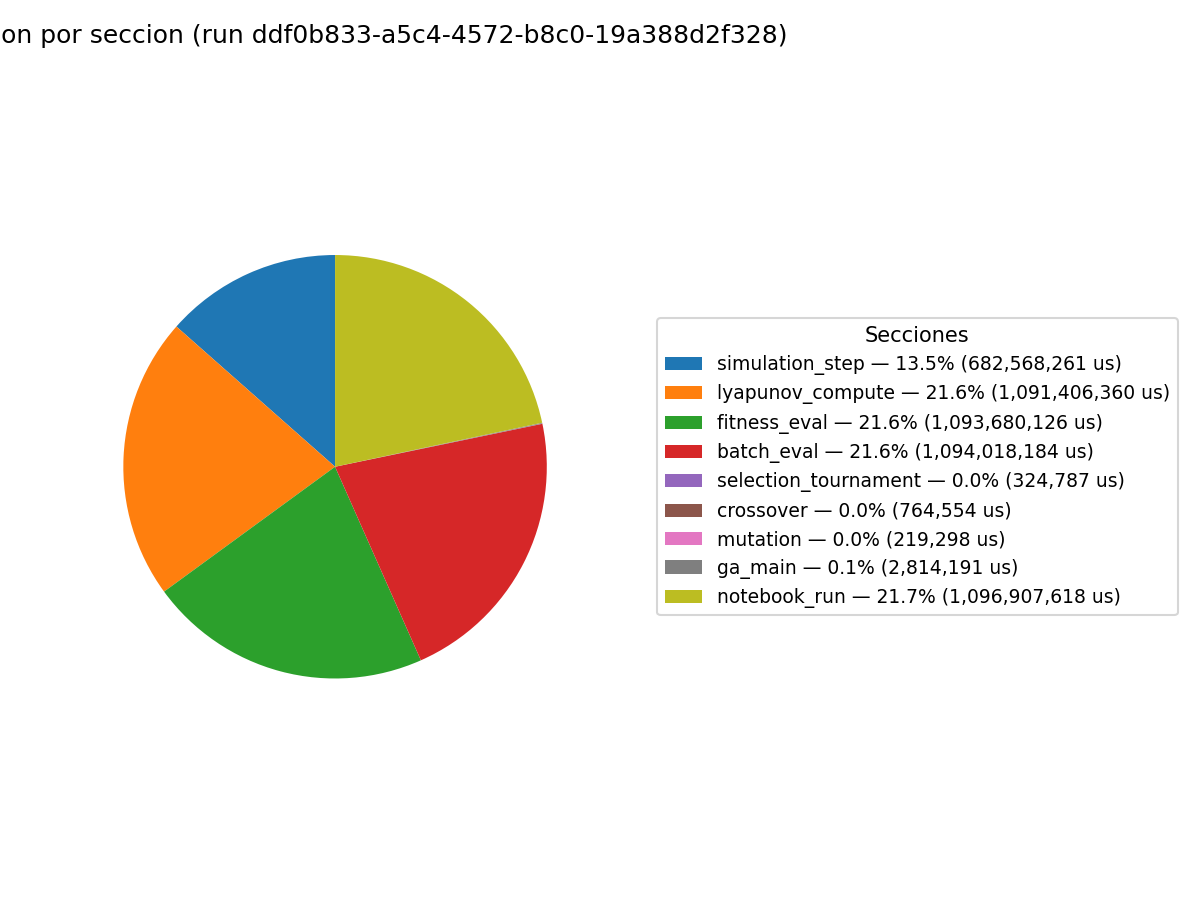
\includegraphics[width=0.85\textwidth]{img/resultados/caso04-metricasTiempo.png}
\caption{Resumen visual del CSV de timings del Caso 04.}
\label{fig:c04_timings} %chktex 24
\end{figure}

\paragraph{D. Resultados y salidas destacadas}
El algoritmo reduce el exponente de Lyapunov corto de $-2.81$ a $-6.01$, incrementando el fitness a $5.46$.\ Las trayectorias optimizadas muestran un intruso menos errante, capaz de permanecer capturado por la binaria durante el horizonte largo.\ Las gráficas de convergencia (\texttt{img/resultados/caso04\_lambda.png}, \texttt{img/resultados/caso04\_fitness.png}) y la vista planar (\texttt{img/resultados/caso04\_planar.png}) constituyen los principales artefactos visuales.

\paragraph{E. Conclusiones del caso}
El intruso rasante obliga al optimizador a explorar masas elevadas para la binaria ($m_1 \approx 1.374$, $m_2 \approx 0.608$) y un intruso de $0.263$ M$_\odot$, combinación que mitiga la divergencia pese a los impulsos iniciales agresivos.
